\documentclass[a4paper, 11pt, normalem]{report}

\usepackage{../../../LaTeX-Templates/Notes}
\usepackage{subfiles}

\title{Advanced Theoretical Physics \vspace{-20pt}}
\author{Dr Kendon and Prof Gardiner}
\date{\vspace{-15pt}Michaelmas Term 2019 - Epiphany Term 2020}
\rhead{\hyperlink{page.1}{Contents}}

\begin{document}

\maketitle
\tableofcontents

\part{Quantum Optics}
\chapter{}
\textbf{Syllabus:}
\begin{multicols}{2}
\begin{itemize}
    \item quantization of light
    \item creation and annihilation operators
    \item Hamiltonian of the E field
    \item number states
    \item coherent states
    \item squeezed states
    \item photon bunching and anti-bunching
    \item density operator
    \item pure states, mixed sates, entangled states
    \item decoherence
    \item atom-light interactions
    \item applications
\end{itemize}
\end{multicols}

\begin{figure}[H]
    \centering
    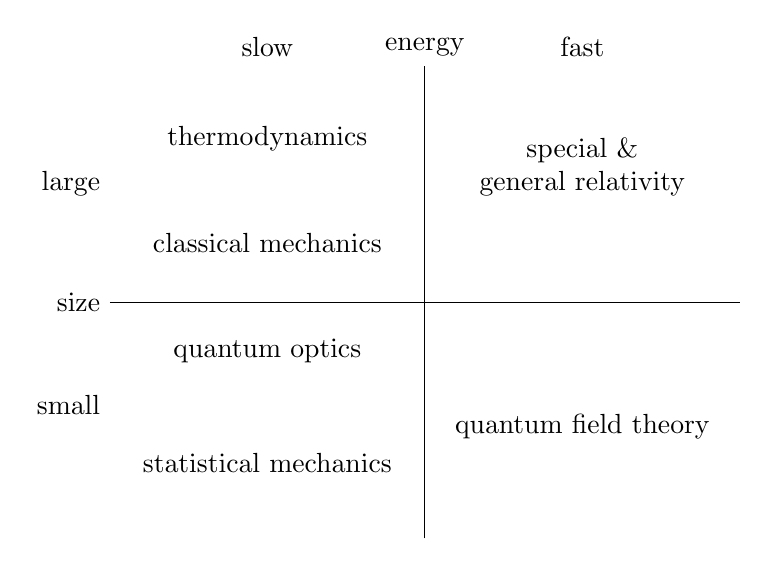
\begin{tikzpicture}
        \draw (-4,0) node[anchor=east] {size} -- (4,0);
        \draw (0,-3) -- (0,3) node[anchor=south] {energy};
        \draw[white] (-2.1,3) -- (-1.9,3) node[black,midway,anchor=south] {slow};
        \draw[white] (1.9,3) -- (2.1,3) node[black,midway,anchor=south] {fast};
        \draw[white] (-4,1.5) node[black,anchor=east] {large} -- (-3.9,1.5);
        \draw[white] (-4,-1.3) node[black,anchor=east] {small} -- (-3.9,-1.3);
        \draw[white] (-2.1,-0.35) -- (-1.9,-0.35) node[black,midway,anchor=north,align=center] {quantum optics};
        \draw[white] (-2.1,-1.8) -- (-1.9,-1.8) node[black,midway,anchor=north,align=center] {statistical mechanics};
        \draw[white] (-2.1,1.8) -- (-1.9,1.8) node[black,midway,anchor=south,align=center] {thermodynamics};
        \draw[white] (1.9,2.2) -- (2.1,2.2) node[black,midway,anchor=north,align=center] {\shortstack{special \&\\general relativity}};
        \draw[white] (1.9,-1.3) -- (2.1,-1.3) node[black,midway,anchor=north,align=center] {quantum field theory};
        \draw[white] (-2.1,0.5) -- (-1.9,0.5) node[black,midway,anchor=south,align=center] {classical mechanics};
    \end{tikzpicture}
\end{figure}

\textbf{Ingredients:}
\begin{itemize}
    \item harmonic oscillators
    \item Gaussian integrals
    \item Hamiltonian mechanics (canonical variables q and p)
    \item maths of operators - adjoint, self-adjoint, Hermitian, commutation relations
    \item QM in both Schrodinger and Heisenberg pictures
    \item density matrices
    \item classical EM - Maxwell's equations in Coulomb gauge - especially plane waves and dipoles
\end{itemize}

Hanbury Brown and Tiss:
\begin{equation}
    G(\tau) = I_A(t)I_B(t+\tau)
\end{equation}

\end{document}















